\documentclass{article}
\usepackage[utf8]{inputenc}
\usepackage{amstext}
\usepackage{amsmath} 
\usepackage{mathpazo}
\usepackage{graphicx} 
\usepackage{float} 
\usepackage{caption} 
\usepackage{epstopdf} 
\usepackage{hyperref}
\usepackage{varioref} 
\usepackage{fancyref}
\usepackage[section]{placeins} 
\usepackage{perpage}
\usepackage[margin=1in, paperwidth=8.5in, paperheight=11in]{geometry} 
\MakeSorted{figure} 
\usepackage{natbib}
\usepackage{graphicx}
\usepackage{xcolor}
\usepackage{listings}
\usepackage{minted}
\usepackage{subcaption}
\usepackage{eso-pic}
\usepackage{tikz}
\usepackage[american]{circuitikz}
\usepackage[font=small,labelfont=bf]{caption}

\title{ENGR2420 Lab 5 : MOS Transistor Characteristics}
\author{Abigail Fry \\ Anusha Datar \\ Vienna Scheyer}
\date{April 1, 2019}

\begin{document}

\maketitle

\section{Experiment One : Gate Characteristics}
In the first experiment, we measured the change in the channel current as a function of gate voltage for both nMOS and pMOS transistors. For the nMOS transistor, we set source voltage to ground and the drain voltage to 5 Volts and then varied the gate voltage from 0 to 5 Volts and measured the current at the source. For the pMOS transitor, we set the source voltage to 5 Volts, set the drain voltage to ground, and then varied the gate voltage from 0 to 5 Volts and measured the current at the drain. 
\begin{figure}[H]   
  \begin{center}       
  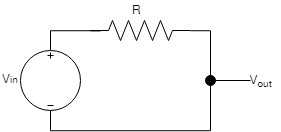
\includegraphics[scale = 0.5]{images/exp1_schematic.jpg}
  \caption{Schematics for the circuits used to measure the current response to changes in gate voltage for nMOS and pMOS transistors.}   
  \label{fig:exp1_sch}
  \end{center}
\end{figure}

\subsection{Results}
Based on this model, we can plot the experimental and theoretical current response to gate voltage for each transistor on semilogarithmic axes. 
\begin{figure}[H]   
  \begin{center}      
  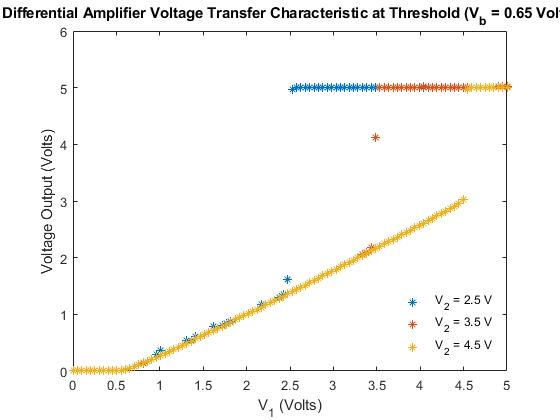
\includegraphics[scale = 0.6]{images/exp1_plot1.jpg}
  \caption{Channel Current-Gate Voltage Plot for nMOS and pMOS transistors.}
  \label{fig:exp1_plot1}
  \end{center}
\end{figure}

Then, we can determine the incremental transconductance gain of the pMOS and nMOS transistors and plot the experimental and theoretical values on log-log axes.
\begin{figure}[H]   
  \begin{center}       
  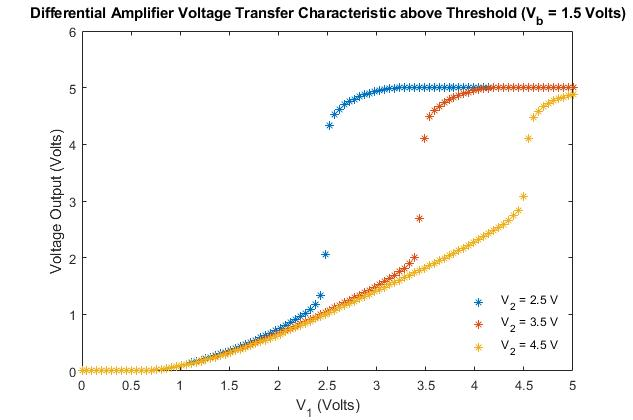
\includegraphics[scale = 0.5]{images/exp1_plot2.jpg}
  \caption{Incremental Transconductance Gain as a function of a current for nMOS and pMOS transistors.}
  \label{fig:exp1_plot1}
  \end{center}
\end{figure}

\subsection{Analysis}
When using the EKV model to characterize the relationship of the channel current and the gate voltage, we assume that the channel current is equal to the saturation current. The value of the saturation current from the pMOS transistor, as shown in the prelab assignmment, is: 
\begin{center}
 $I_{sat} = I_{s}log^{2}{(1 + e^{\frac{\kappa(V_G - V_{T0}) - V_S)}{2U_T}}})$
\end{center}

\noindent The value of the saturation current from the pMOS transistor, as shown in the prelab assignmment, is: 
\begin{center}
 $I_{sat} = I_{s}log^{2}{(1 + e^{\frac{\kappa((V_{DD} - VG) - V_{T0}) - (V_{DD} - V_S)}{2U_T}}})$
\end{center}

By using the ekvfit function in MATLAB (with epsilon value 5e-7), we were able to extract values of $I_s$, $\kappa$, and $V_{T0}$ for each type of transistor. For the nmos transistor, the value of $I_s$ was $2.1307*10^{-7}$ Amps, $\kappa$ was $.556$, and $V_{T0}$ was $.588$ Volts. For the pMOS transistor, the value of $I_s$ was $5.288*10^{-7}$ Amps, $\kappa$ was $.81535$, and $V_{T0}$ was $.62255$ Volts. Note that because $\kappa$ is a divider ratio, it is a dimensionless quantity.

We then could compare our theoretical model of each transistor to the data we collected in the lab. In general, our plots qualitatively match expected  values. Note that there is some noise at high voltages for the pMOS and low voltages for the nMOS - this is likely due to the difficulties associated with measuring very low currents using the SMU. Furthermore, the actual theoretical fits are based on calculations associated with careful sampling of the current data, so any overepresentation or underrepresentation of specific regions in the points used to extract the parameters for the model could lead to deviations in the plot.

We also extracted the incremental transconductance gain for both transistors. In theory the incremental transconductance gain is equal to the ratio between the change in channel current and the change in voltage at the gate. In the case of the nMOS transistor, this implies that the transconductance gain, or $g_m$ is equal to $\frac{\kappa}{U_T}*\sqrt{I_sI_{sat}} * (1 - e^{-\sqrt{I_sI_{sat}}}$, In the weak inversion case (when $I_{sat} << I_s$), this generalizes to $\frac{\kappa}{U_T}*I_{sat}$, and in the strong inversion case (when $I_{sat} >> I_s$), this generalizes to $\frac{\kappa}{U_T}*\sqrt{I_sI_{sat}}$. In the case of the pMOS transistor, this relationship is inverted - $g_m$ is equal to $-\frac{\kappa}{U_T}*\sqrt{I_sI_{sat}} * (1 - e^{-\sqrt{I_sI_{sat}}})$. In the weak inversion case (when $I_{sat} << I_s$), this generalizes to $-\frac{\kappa}{U_T}*I_{sat}$, and in the strong inversion case (when $I_{sat} >> I_s$), this generalizes to $-\frac{\kappa}{U_T}*\sqrt{I_sI_{sat}}$. These two curves should intersect at $I_s$.

Experimentally, we calculated incremental transconductance gain by calculating the quotient of the partial derivative of the channel current for each transistor and the partial derivative of the gate voltage for each transistor. To do this, we leveraged MATLAB's $diff$ function and calculated the value of the transconductance at each point.

Again, both the theoretical and experimental plots qualitatively resemble each other - notably, each of the experimental and theoretical plots have distinct weak-inversion and strong-inversion regions with an inflection point around the extracted value of $I_s$. Like the prior plot, this example is subject to issues associated with low current values and the points sampled when extracting the parameters.

\subsection{Discussion}
The theoretical fits match the data in both the weak-inversion and strong-inversion regions. This is the case for both the general current-voltage plot and for the transconductance plot - however, there tends to be variation at low current values (most notably in the pMOS weak inversion case), which is likely due to measurement difficulties at low currents. 

\section{Experiment Two : Source Characteristics}
In the second experiment, we measured the change in the channel current as a function of source voltage for both nMOS and pMOS transistors. For the nMOS transistor, we set both the gate and the drain voltage to 5 Volts and then varied the source voltage from 0 to 5 Volts and measured the current at the source. For the pMOS transitor, we set both the source and drain voltage to ground and then varied the source voltage from 0 to 5 Volts and measured the current at the drain. 

\begin{figure}[H]   
\begin{center}
  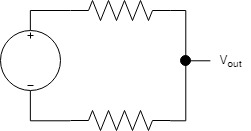
\includegraphics[scale = 0.5]{images/exp2_schematic.jpg}
  \caption{Schematics for the circuits used to measure the current response to changes in source voltage for nMOS and pMOS transistors.}   
  \label{fig:exp2_sch}
  \end{center}

\end{figure}

\subsection{Results}
We first plotted the source voltage - channel current characteristics for the transistors. Then, we used the $linefit$ function to create source characteristics for the nMOS and pMOS devices on semilogarithmic axes.  
\begin{figure}[H]   
  \begin{center}       
  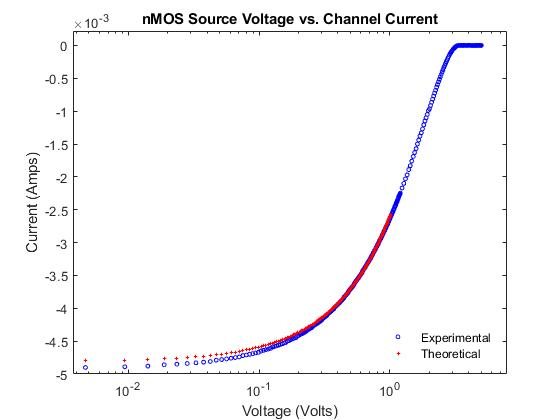
\includegraphics[scale = 0.5]{images/s_nMOS.jpg}
  \caption{Source characteristic for the nMOS transistor.}   
  \label{fig:sp}
  \end{center}
\end{figure}

\begin{figure}[H]   
  \begin{center}       
  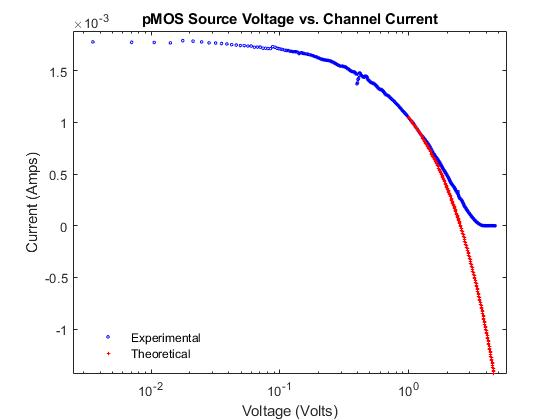
\includegraphics[scale = 0.5]{images/s_pMOS.jpg}
  \caption{Source characteristic for the pMOS transistor.}   
  \label{fig:np}
  \end{center}
\end{figure}

Then, we extracted the incremental source conductance at weak inversion and strong inversion for the two types of transistors and plotted the values on a loglog scale.

\begin{figure}[H]   
  \begin{center}       
  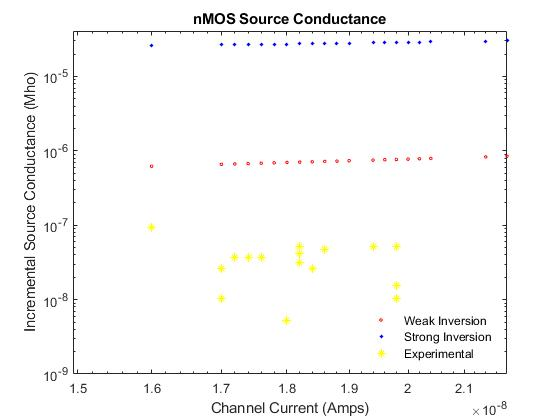
\includegraphics[scale = 0.5]{images/sc_nMOS.jpg}
  \caption{Incremental Source conductance as a function of channel current for nMOS.}   
  \label{fig:n_sc}
  \end{center}
\end{figure}

\begin{figure}[H]   
  \begin{center}       
  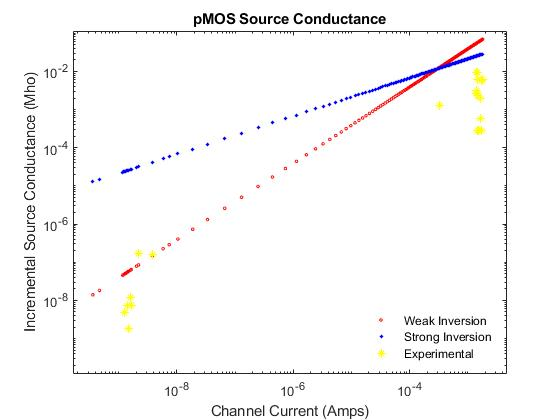
\includegraphics[scale = 0.5]{images/sc_pMOS.jpg}
  \caption{Incremental Source conductance as a function of channel current for pMOS.}   
  \label{fig:p_sc}
  \end{center}
\end{figure}
\subsection{Analysis}
To find the theoretical fit at the weak inversion region for the nMOS and pMOS source characteristic, we used the $linefit$ function provided with the lab.  We used the epsilon value $5e^{4}$ recommended in the function to get to a line of best-fit.  We then plotted the fit to the weak inversion region for each transistor.
\newline
\newline
To plot the experimental incremental source conductance for the nMOS and pMOS transistors we used 
\begin{center}
 $g_{m_{exp}} = \frac{\partial I_{sat}}{\partial V_{S}}$
\end{center}
where $g_{m_{exp}}$ is experimental source conductance,$V_{S}$ is source voltage in Volts, and $I_{sat}$ is channel current in Amps.  In $MATLAB$, we used $diff$ and ./ to create the experimental plots.  The theoretical fits for the nMOS and pMOS are the same. For the weak inversion region, both transistor fits can theoretically be represented with
\begin{center}
$ g_{m_{w}} =\frac{I_{sat}}{U_{t}}$
\end{center}
where $ g_{m_{w}}$ is theoretical source conductance in weak inversion and $U_{t}$ is the thermal voltage constant at .0258 Volts.  This value was provided in $ekvfit$ function that came with the lab.  In the strong inversion region, both transistors can theoretically be represented with 
\begin{center}
$ g_{m_{s}} =\frac{\sqrt{I_{s}I_{sat}}}{U_{t}}$
\end{center}
here $ g_{m_{s}}$ is theoretical source conductance in strong inversion region and $I_{s}$ is 2 times the constant threshold current at the transition point defined in the source characteristic.  For this lab, the transition point was between the qualitatively found ohmic and saturation regions.
\subsection{Discussion}
The source characteristics of both transistors have distinct weak-inversion and strong-inversion regions with an inflection point around the extracted value of $I_{s}$.
The slope of the exponential region in Figure \ref{fig:sp} is 0.0022 (Mho) and the slope of the exponential region in Figure \ref{fig:np} is -6.849e-04 (Mho). 
The voltage- channel current characteristic at the source follow similar trends as the voltage - channel current characteristics at the gate from  Experiment One. For the nMOS transistor, as the Voltage at the source increases, so does the channel current - it first increases exponentially and then linearly. Meanwhile, for the pMOS transistor, as the voltage at the source increases, the channel current decreases - first exponentially and then linearly. 
\newline
We did have some challenges with Figure \ref{fig:n_sc}.  The weak and strong inversion lines should intersect each other similarly to how the lines intersect in Figure \ref{fig:p_sc}.  Weak inversion and strong inversion have very few data points shown compared to Figure \ref{fig:p_sc}. This issue persisted when we re-collected data, and we were unable to resolve it computationally.
\section{Experiment Three : Drain Characteristics}
In Experiment 3, we measured the channel current as a function of drain voltage while holding the gate voltage at three different values for both an nMOS and a pMOS transistor.
\begin{figure}[H]   
  \centering        
  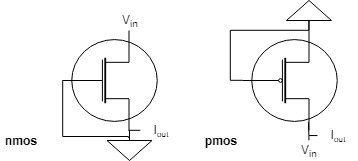
\includegraphics[scale = 0.5]{images/exp3_schematic.jpg}
  \caption{Schematics for the circuits used to measure the current response to changes in drain voltage for nMOS and pMOS transistors.}   
  \label{fig:exp2_sch}
\end{figure}

\subsection{Results}

Figure \ref{fig:nMOS_char} shows the drain characteristics of an nMOS transistor. We held the gate voltage at three constant values: 100 mV below the threshold voltage (0.6 V) for weak inversion, the threshold voltage (0.7 V) for moderate inversion, and $V_{dd}$ (5 V) for strong inversion. 
\begin{figure}[H]   
  \centering      
  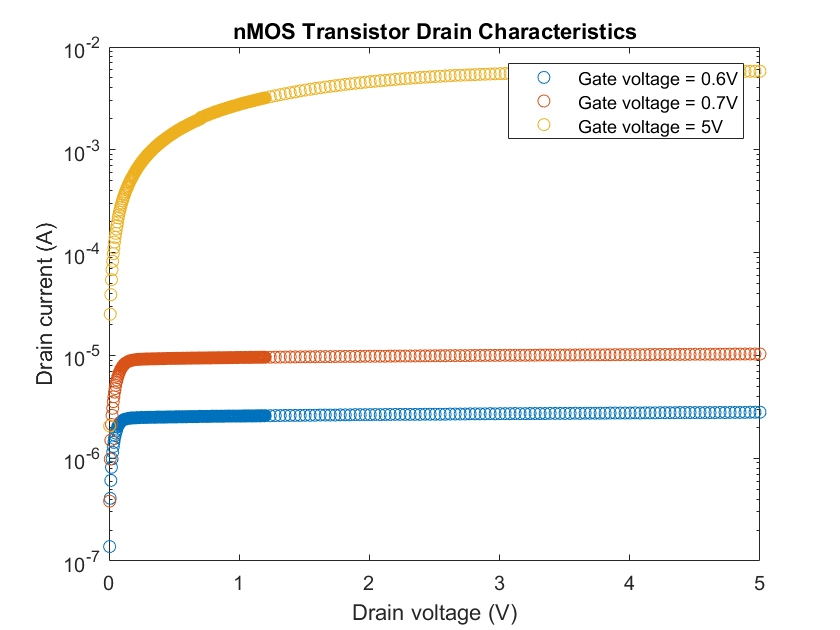
\includegraphics[scale = 0.5]{images/nMOS_drain_characteristics.png}
  \caption{nMOS drain characteristics. }   
  \label{fig:nMOS_char}
\end{figure}

Figure \ref{fig:pMOS_char} shows the drain characteristics of a pMOS transistor. We held the gate voltage at three constant values: 100 mV above the threshold voltage (4.3 V) for weak inversion, the threshold voltage (4.2 V) for moderate inversion, and ground (0 V) for strong inversion. 

\begin{figure}[H]   
  \centering        
  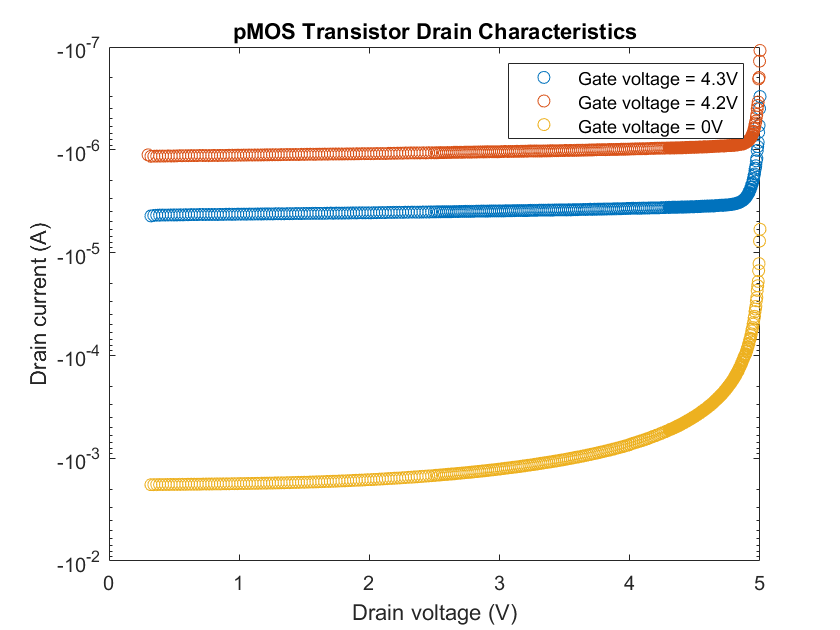
\includegraphics[scale = 0.5]{images/pMOS_drain_characteristics.png}
  \caption{pMOS drain characteristics}   
  \label{fig:pMOS_char}
\end{figure}

Figure \ref{fig:early} shows a semilogarithmic plot of Early voltage as a function of saturation current (x-axis logarithmic) for all three gate voltages for both the nMOS and pMOS transistor.

\begin{figure}[H]   
  \centering        
  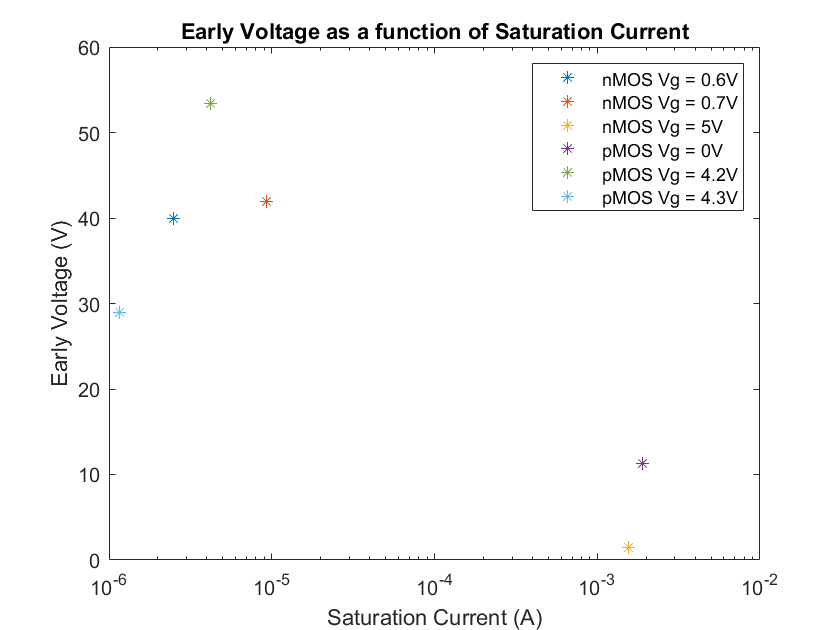
\includegraphics[scale = 0.5]{images/early_voltage.png}
  \caption{nMOS Early Voltage}   
  \label{fig:early}
\end{figure}

Figure \ref{fig:gsro} shows a loglog plot of intrinsic gain ( $g_s$ ) as a function of saturation current for all three gate voltages for both the nMOS and pMOS transistor.

\begin{figure}[H]   
  \centering        
  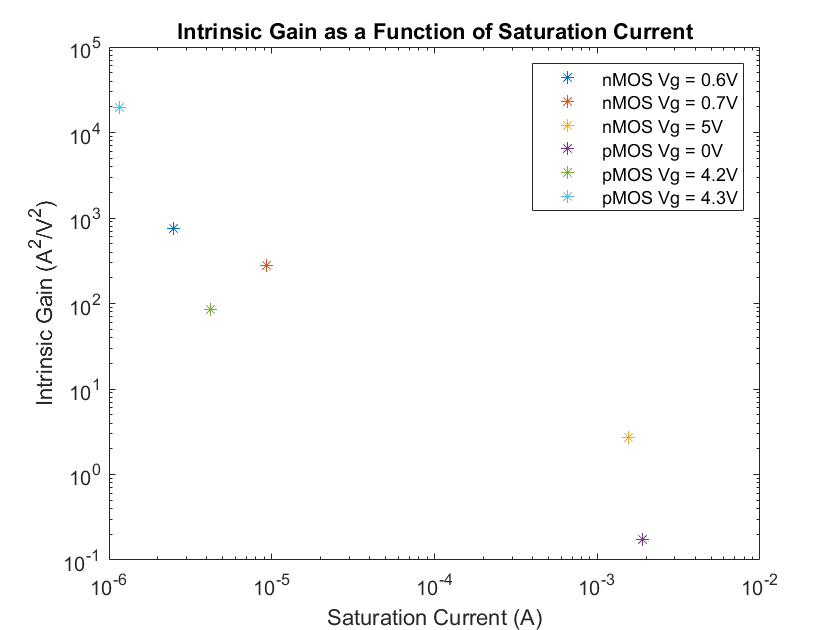
\includegraphics[scale = 0.5]{images/gsro.png}
  \caption{pMOS Early Voltage as a function of saturation current}   
  \label{fig:gsro}
\end{figure}

\subsection{Analysis}
\flushleft
To extract saturation current for each transistor, we used the MATLAB $polyfit$ function to fit a line to the saturation region at each gate voltage. The saturation current is the y-intercept of this best fit line, so we took the y-intercept of the $polyfit$ to get saturation current.
To extract Early voltage, we used the equation
\begin{centering}
$$VA = r_o I_{sat}$$
\end{centering}

In order to use that equation we also needed to extract $r_o$ which we did by taking the inverse of the slope in the saturation region. 

To extract intrinsic gains for each transistor, we had to extract incremental source conductance, $g_s$. To extract $g_s$, we used the $polyfit$ function to fit a line to the ohmic region for each gate voltage. The slope of this best fit line is equal to $g_s$. Then we multiplied to get intrinsic gain, $g_s r_o$. Table \ref{tab:nMOS_vals} shows the extracted values for the nMOS transistor at three gate voltages, and Table \ref{tab:pMOS_vals} shows the extracted values for the pMOS transistor at three gate voltages.

\begin{table}[h]
    \begin{centering}
    \begin{tabular}{|c|c|c|c|}
        \hline
         Gate Voltage (V) & Saturation Current (A) & Early Voltage (V) & Intrinsic Gain (mhos^{2}) \\ \hline
        0.6 & 2.51 x 10^{-6} & 39.94 & 758 \\ \hline
        0.7 & 9.30 x 10^{-6} & 41.93 & 282 \\ \hline
        5 & 1.56 x 10^{-3} & 1.42 & 2.74 \\ \hline
    \end{tabular}
    \caption{Extracted values for nMOS transistor}
    \label{tab:nMOS_vals}
    \end{centering}
\end{table}

\begin{table}[h]
    \begin{centering}
    \begin{tabular}{|c|c|c|c|}
        \hline
         Gate Voltage (V) & Saturation Current (A) & Early Voltage (V) & Intrinsic Gain (mhos^{2}) \\ \hline
        0 & -1.89 x 10^{-3} & -11.31 & 0.17 \\ \hline
        4.2 & -4.23 x 10^{-6} & -53.37 & 84.66 \\ \hline
        4.3 & -1.17 x 10^{-6} & -28.89 & 1.95 x 10^{4} \\ \hline
    \end{tabular}
    \caption{Extracted values for pMOS transistor}
    \label{tab:pMOS_vals}
    \end{centering}
\end{table}
\newpage
\subsection{Discussion}
In weak and moderate inversion regions for both nMOS and pMOS transistors, the intrinsic gain is much greater than unity, so in weak and moderate inversion regions it would be appropriate to assume that the transistor's intrinsic gain will be much larger than unity. For the strong inversion case, however, the intrinsic gains are $2.74 Mhos^2$ and $0.17 Mhos^2$ for nMOS and pMOS respectively. The nMOS value is fairly close to unity and the pMOS value is less than unity, so in the strong inversion region this assumption would not generally hold true.
\end{document}
